\begin{enumerate}[label=\thesubsection.\arabic*,ref=\thesubsection.\theenumi]
\item  The cable of a uniformly loaded suspension bridge hangs in the form of a parabola. The roadway which is horizontal and 100 m long is supported by vertical wires attached to the cable, the longest wire being 30 m and the shortest being 6 m. Find the length of a supporting wire attached to the roadway 18 m from the middle.
\label{chapters/11/11/5/3}
\\
\solution
		Rewriting \eqref{eq:chapters/11/11/5/6/parabola} in matrix form,
    \begin{align}
        \vec{x}^\top\myvec{1&0\\0&0}\vec{x} + 2\myvec{0&-6}\vec{x} = 0
        \label{eq:chapters/11/11/5/6/parabola-mtx}
    \end{align}
    The above parabola can be  expressed in standard form using 
\begin{align}
	\vec{x} = \vec{P}\vec{y} = \myvec{0 & 1 \\ 1 & 0}\vec{y}
        \label{eq:chapters/11/11/5/6/affine}
\end{align}
yielding
    \begin{align}
        \vec{y}^\top\myvec{0&0\\0&1}\vec{x} + 2\myvec{-6&0}\vec{x} = 0
        \label{eq:chapters/11/11/5/6/parabola-mty}
    \end{align}
    Hence, 
    from
\eqref{eq:conic_quad_form_nc}, 
    \begin{align}
	    \vec{n} = \vec{e}_1
        \label{eq:chapters/11/11/5/6/n}
	\\
	    c = -\frac{36}{2\times 6} = -3
    \end{align}
    Substituting in 
  \eqref{eq:conic_quad_form_F} 
  yields
    \begin{align}
        \vec{F} = 3\vec{e}_1
    \end{align}
    Thus, the equation of the latus rectum is
\begin{align}
        \vec{x} = \vec{F} + \kappa \vec{e}_2
        \label{eq:chapters/11/11/5/6/x-general}
    \end{align}
        Substituting in \eqref{eq:chapters/11/11/5/6/parabola-mty} and simplifying,
    \begin{align}
\kappa = \pm 6
        \label{eq:chapters/11/11/5/6/x-latus}
    \end{align}
    Thus, the ends of the latus rectum are
    \begin{align}
        \vec{y} = \myvec{3 \\ \pm 6}
    \end{align}
    The relevant parameters with respect to 
        \eqref{eq:chapters/11/11/5/6/parabola-mtx}
	can now be obtained using 
        \eqref{eq:chapters/11/11/5/6/affine}.
See \figref{fig:chapters/11/11/5/6/parabola}.
The area of the required triangle is
    \begin{align}
        \textrm{ar}\brak{\triangle OAB} = \frac{1}{2}\mydet{6&3\\-6&3} = 18 
    \end{align}
    \begin{figure}[H]
        \centering
        %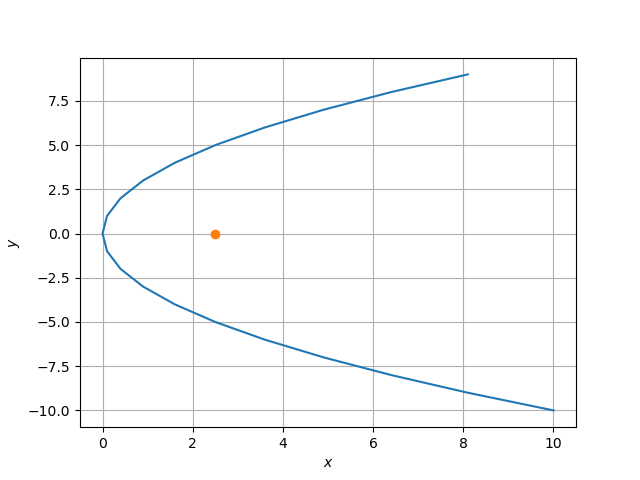
\includegraphics[width=0.75\columnwidth]{chapters/11/11/5/6/figs/parabola.png}
        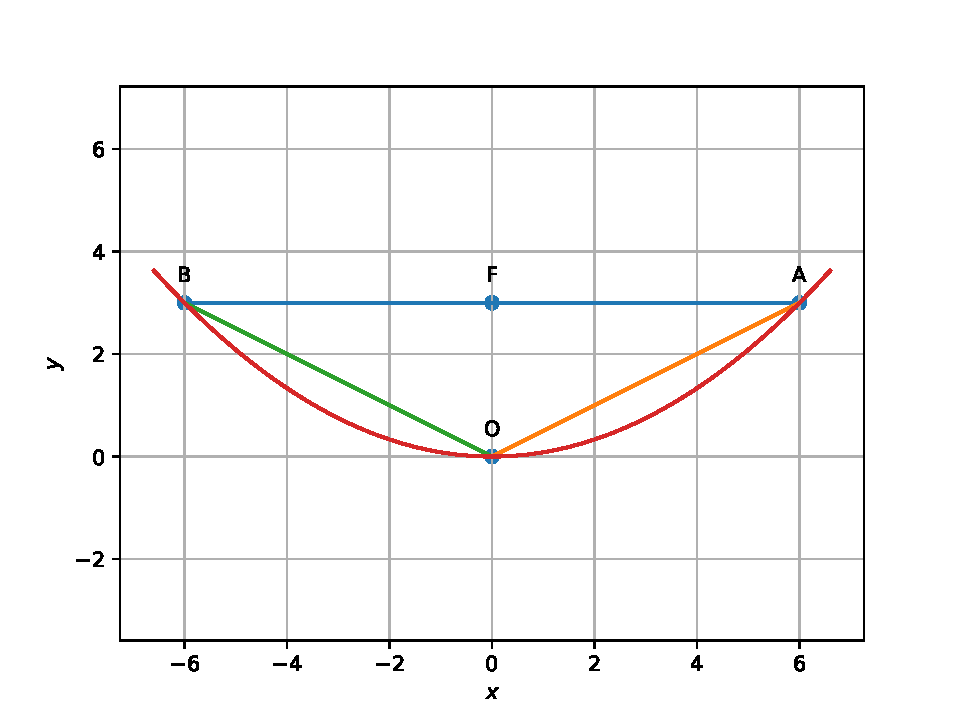
\includegraphics[width=0.75\columnwidth]{chapters/11/11/5/6/figs/fig1.pdf}
        \caption{}
        \label{fig:chapters/11/11/5/6/parabola}
    \end{figure}

    \item Find the area of the triangle formed by the lines joining the vertex 
    of the parabola 
    \begin{align}
        x^2 = 12y
        \label{eq:chapters/11/11/5/6/parabola}
    \end{align}
    to the ends of its latus rectum.
\label{chapters/11/11/5/6}
\\
\solution
		Rewriting \eqref{eq:chapters/11/11/5/6/parabola} in matrix form,
    \begin{align}
        \vec{x}^\top\myvec{1&0\\0&0}\vec{x} + 2\myvec{0&-6}\vec{x} = 0
        \label{eq:chapters/11/11/5/6/parabola-mtx}
    \end{align}
    The above parabola can be  expressed in standard form using 
\begin{align}
	\vec{x} = \vec{P}\vec{y} = \myvec{0 & 1 \\ 1 & 0}\vec{y}
        \label{eq:chapters/11/11/5/6/affine}
\end{align}
yielding
    \begin{align}
        \vec{y}^\top\myvec{0&0\\0&1}\vec{x} + 2\myvec{-6&0}\vec{x} = 0
        \label{eq:chapters/11/11/5/6/parabola-mty}
    \end{align}
    Hence, 
    from
\eqref{eq:conic_quad_form_nc}, 
    \begin{align}
	    \vec{n} = \vec{e}_1
        \label{eq:chapters/11/11/5/6/n}
	\\
	    c = -\frac{36}{2\times 6} = -3
    \end{align}
    Substituting in 
  \eqref{eq:conic_quad_form_F} 
  yields
    \begin{align}
        \vec{F} = 3\vec{e}_1
    \end{align}
    Thus, the equation of the latus rectum is
\begin{align}
        \vec{x} = \vec{F} + \kappa \vec{e}_2
        \label{eq:chapters/11/11/5/6/x-general}
    \end{align}
        Substituting in \eqref{eq:chapters/11/11/5/6/parabola-mty} and simplifying,
    \begin{align}
\kappa = \pm 6
        \label{eq:chapters/11/11/5/6/x-latus}
    \end{align}
    Thus, the ends of the latus rectum are
    \begin{align}
        \vec{y} = \myvec{3 \\ \pm 6}
    \end{align}
    The relevant parameters with respect to 
        \eqref{eq:chapters/11/11/5/6/parabola-mtx}
	can now be obtained using 
        \eqref{eq:chapters/11/11/5/6/affine}.
See \figref{fig:chapters/11/11/5/6/parabola}.
The area of the required triangle is
    \begin{align}
        \textrm{ar}\brak{\triangle OAB} = \frac{1}{2}\mydet{6&3\\-6&3} = 18 
    \end{align}
    \begin{figure}[H]
        \centering
        %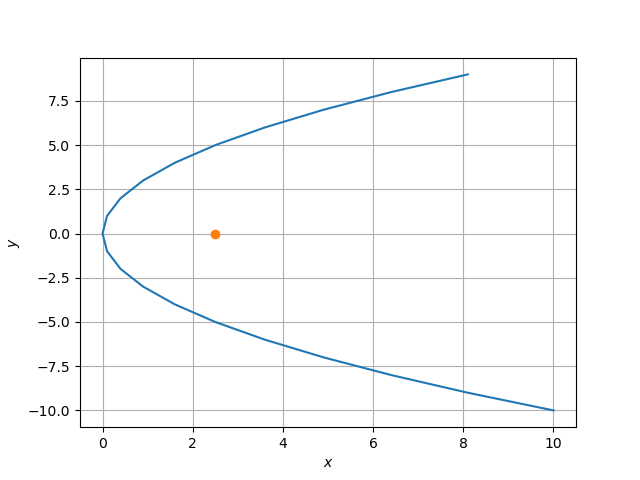
\includegraphics[width=0.75\columnwidth]{chapters/11/11/5/6/figs/parabola.png}
        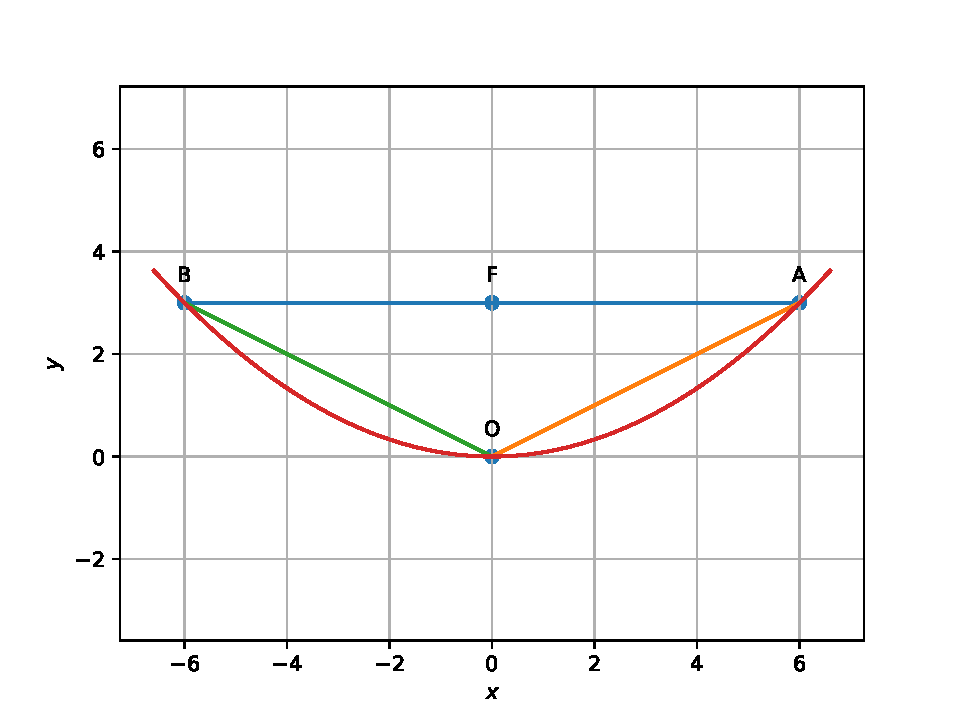
\includegraphics[width=0.75\columnwidth]{chapters/11/11/5/6/figs/fig1.pdf}
        \caption{}
        \label{fig:chapters/11/11/5/6/parabola}
    \end{figure}

\item A man running a racecourse notes that the sum of the distances from the two flag posts from him is always 10 m and the distance between the flag posts is 8 m. Find the equation of the posts traced by the man. 
\label{chapters/11/11/5/7}
 \item Find the coordinates of a point on the parabola $y^2=8x$ whose focal distance is 4.
\item Show that the set of all points such that the difference of their distances from (4,0) and (-4,0) is always equal to 2 represent a hyperbola.
\item If the distance between the foci of a hyperbola is 16 and its eccentricity is $\sqrt{2}$, then obtain the equation of the hyperbola.
\item The eccentricity of the hyperbola whose latus rectum is 8 and conjugate axis is equal to half of the distance between the foci is 
\begin{enumerate}
\item $\frac{4}{3}$
\item $\frac{4}{\sqrt{3}}$
\item $\frac{2}{\sqrt{3}}$
\item none of these
\end{enumerate}
\item The distance between the foci of a hyperbola is 16 and its eccentricity is $\le{2}$. lts equation is
\begin{enumerate}
\item $x^2-y^2=3^2$
\item $\frac{x^2}{4-}\frac{y^2}{9}=1$
\item $2x-3y^2=7$
 \item none of these
 \end{enumerate}
 \item If the latus rectum of an ellipse is equal to half of minor axis, then find its eccentricity.
 \item If the eccentricity of an ellipse is $\frac{5}{8}$ and  the distance between its foci is 10 then find latus rectum of the ellipse.
 \item Find the distance between the directrices of the ellipse $\frac{x^2}{36}+\frac{y^2}{20}$
\item Find the equation of the set of all points the sum of whose distances  from the points (3,0) and (9,0) is 12.
\item If ${P}$ is a point on the ellipse $\frac{x^2}{16}+\frac{y^2}{25}=1$ whose foci  are $s$ and $s'$ then $Ps +Ps'=8$.
\item An arch is in the form of a parabola with its axis vertical. The arch is 10m high and 5m wide at the base. How wide is it 2m from the vertex of the parabola?
\label{chapters/11/11/5/2}
\item An equilateral triangle is inscribed in the parabola $y^{2} = 4ax$,where one vertex is at the vertex of the parabola. Find the length of the side of the triangle.
\label{chapters/11/11/5/8}
\item An arch is in the form of a semi-ellipse. It is 8 m wide and 2 m high at the centre. Find the height of the arch at a point 1.5 m from one end.
\label{chapters/11/11/5/4}
\item A rod of length 12cm moves with its ends always touching the coordinate axes. Determine the equation of locus of a point  P on the rod, which is 3cm from the end in contact with $x-axis$.
\label{chapters/11/11/5/5}
\end{enumerate}
